\section{Durchführung}
\label{sec:Durchführung}
\subsection{Bestimmung des Schubmoduls $G$}
    \begin{figure}
        \centering
        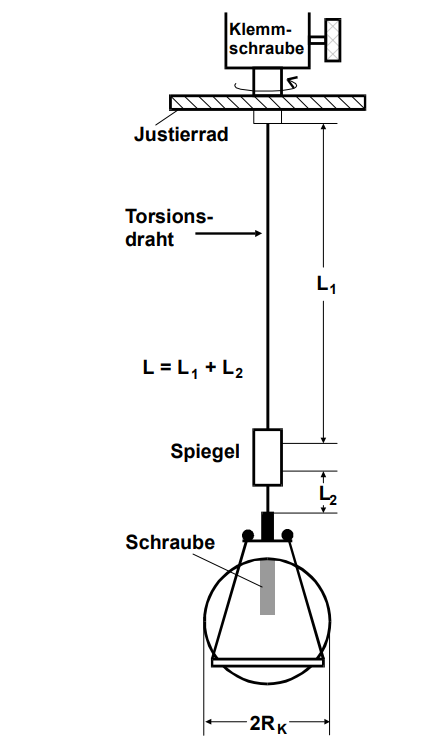
\includegraphics[width=\textwidth]{content/aufbau.png}
        \caption{Aufbau der Messaparatur \cite[100]{V102}.}
        \label{fig:aufbau}
    \end{figure}
    Das Schubmodul $G$ wird mittels des in des \autoref{fig:aufbau} dargestellten Aufbaus ermittelt.
    Hierzu wird die Vorrichtung durch Betätigung des Justierrades leicht ausgelenkt, so dass sie eine Drehbewegung um die eigene
    Achse vollführt. Zu Beachten ist dabei, dass die Kugel wirklich nur die Drehbewegung vollführt; andere Schwingungen können
    das Ergbenis beeinflussen und verfälschen.
    Die Schraube in der Kugel markiert die Ausrichtung des Permanentmagneten in der Kugel, dieser soll senkrecht stehen, um den
    Einfluss von diesem (besonders mit Einfluss des Erdmagnetfeldes) möglichst gering ist.
    Der Spiegel sendet immer dann ein Signal an eine Photodiode wenn der Strahl einer Leuchte auf den Spiegel scheint, also zweimal pro
    Periode. Die Photodiode sendet ein Signal an eine digitale Schaltung, welche daraufhin eine Stoppuhr startet. Das nächste Signal 
    wird mittels einer bistabilen Kippstufe unterdrückt, da diese keine Verwendung hat. Das darauffolgende Signal stoppt die Uhr.
    Die angezeigte Zeit wird notiert. Ein erneutes Siganl setzt den Zähler zurück. Die Messaufnahme wird insgesamt zehnmal durchgeführt
    und anschließend wird über die angezeigten Zeiten gemittelt.
\subsection{Bestimmung des magnetischen Momentes} 
    Der zuvor verwendete Versuchsaufbau wird beibehalten und erweitert. Zum einen wird ein Helmholtzspulenpaar aufgestellt, welches
    an der Kugel für ein homogenes Magnetfeld sorgt, zum Anderen wird die Kugel so gedreht, dass die Schraube waagerecht ist, um
    den Einfluss des Erdmagnetfeldes zu minimieren. 
    Es wird zuerst eine Stromstärke von $0.5$A angelegt, welche in $0.5$A - Schritten bis 5A erhöht wird. Bei jeder Stromstärke
    werden insgesamt 10 Messungen durchgeführt. Hier ist es nochmal besonders wichtig auf äußere Schwingungen zu achten, da die
    Perioden immer kürzer werden mit zunehmender Stromstärke und kleine Einflüsse so einen vergleichsweise großen Einfluss haben.
